%!TEX root = ../07-Electrical-Components.tex
\chapter{Current-Voltage Characteristics}

\begin{figure}[tbp]
	\centering
	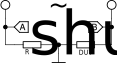
\includegraphics[width=.4\textwidth]{img/sch-iv-curve.pdf}
	\caption{Curve Tracer Schematic}
	\label{sch:curve}
\end{figure}

Current-Voltage Characteristics are recorded first in a quasi-static setup, later at higher frequencies.

\section{Setup}

\section{Evaluation}

\begin{equation*}
	U_\text{f, Si} = \SI{0.58}{\volt}, \qquad U_\text{f, Ge} = \SI{0.33}{\volt}.
\end{equation*}

\def\ivsubfigwidth{0.45\textwidth}
\def\ivgraphicswidth{1.1\textwidth}

\begin{figure}[tbp]
	\centering

	\begin{subfigure}{\ivsubfigwidth}
		\centering
		\includegraphics[width=\ivgraphicswidth]{data/plots/diodes-low-freq.pdf}
		\caption{Si- and Ge-Diode}
		\label{plot:iv:si-ge-diode}
	\end{subfigure}
	\begin{subfigure}{\ivsubfigwidth}
		\centering
		\includegraphics[width=\ivgraphicswidth]{data/plots/z-diode-low-freq.pdf}
		\caption{Z-Diode}
		\label{plot:iv:z-diode}
	\end{subfigure}

	\begin{subfigure}{\ivsubfigwidth}
		\centering
		\includegraphics[width=\ivgraphicswidth]{data/plots/leds-low-freq.pdf}
		\caption{LEDs}
		\label{plot:iv:leds}
	\end{subfigure}
	\begin{subfigure}{\ivsubfigwidth}
		\centering
		\includegraphics[width=\ivgraphicswidth]{data/plots/photodiode-low-freq.pdf}
		\caption{Photodiode}
		\label{plot:iv:photodiode}
	\end{subfigure}

	\caption{$I$-$V$ Curves of Diodes}
	\label{plot:iv:diodes}
\end{figure}

\begin{figure}[tbp]
	\centering

	\begin{subfigure}{\ivsubfigwidth}
		\centering
		\includegraphics[width=\ivgraphicswidth]{data/plots/ldr-low-freq.pdf}
		\caption{LDR}
		\label{plot:iv:ldr}
	\end{subfigure}
	\begin{subfigure}{\ivsubfigwidth}
		\centering
		\includegraphics[width=\ivgraphicswidth]{data/plots/varistor-low-freq.pdf}
		\caption{Varistor}
		\label{plot:iv:varistor}
	\end{subfigure}

	\caption{$I$-$V$ Curves of Resistors}	%sounds exciting, doesn't it?
	\label{plot:iv:boring}
\end{figure}
